\documentclass[12pt]{article}

\usepackage{amsmath}
\usepackage{amssymb}
\usepackage{geometry}
\usepackage{enumitem}
\usepackage{tikz}
\usetikzlibrary{
    arrows.meta,
    calc,
    angles,
    quotes,
    decorations.pathmorphing
}
\usepackage[american]{circuitikz}


\geometry{margin=1in}

\begin{document}

\begin{enumerate}[leftmargin=*]

\item A rectangular conducting loop of width \(4\,\text{cm}\) (radially outward) and height \(6\,\text{cm}\) moves with constant speed \(2\,\text{m/s}\) directly away from a long straight wire carrying steady current \(15\,\text{A}\). At the instant considered, the nearer vertical side is \(2\,\text{cm}\) from the wire and the total loop resistance is \(0.2\,\Omega\). Using exact logarithmic flux evaluation (not uniform-field approximation), determine the instantaneous induced current magnitude.  

% ---------------- Question 1 Diagram ----------------
\begin{tikzpicture}[x=1cm,y=1cm]

% Long straight wire
\draw[thick] (0,0) -- (0,7);
\node[left] at (0,6.8) {Long straight wire};
\node[left] at (0,5.8) {$I=15\,A$};

% Rectangular loop (scaled correctly: 4 cm width, 6 cm height)
\draw[thick] (2,1) rectangle (6,7);
\node[right] at (6,6) {Loop};

% Velocity arrow (shifted to avoid crowding)
\draw[->,thick] (6.8,4) -- (8,4);
\node[right] at (8,4) {$v=2\,m/s$};

% Distance marking (2 cm correct)
\draw[<->] (0,-0.5) -- (2,-0.5);
\node at (1,-0.9) {$2\,cm$};

% Width marking (4 cm correct)
\draw[<->] (2,0.2) -- (6,0.2);
\node at (4,-0.2) {$4\,cm$};

% Height marking (6 cm correct)
\draw[<->] (6.7,1) -- (6.7,7);
\node[right] at (6.7,3) {$6\,cm$};

\end{tikzpicture}

A) \(0.38\,\text{mA}\)  

B) \(0.76\,\text{mA}\)  

C) \(1.52\,\text{mA}\)  

D) \(0.19\,\text{mA}\)  

\item A conducting rod of length \(0.5\,\text{m}\) slides with constant speed \(4\,\text{m/s}\) on parallel rails separated by \(0.5\,\text{m}\) inside a magnetic field \(B(x)=0.6+0.1x\) (SI units), where \(x\) is displacement along motion. The total circuit resistance is \(3\,\Omega\), and the rod is at \(x=0\) at the instant considered. Including first-order correction due to field gradient, the mechanical power required at that instant equals:  

% ---------------- Question 2 Diagram ----------------
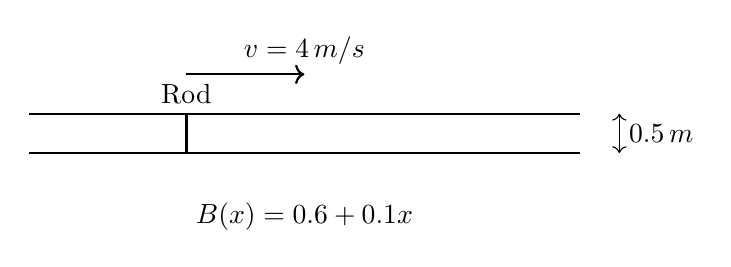
\begin{tikzpicture}[x=1cm,y=1cm]

% Rails (0.5 m separation)
\draw[thick] (0,0) -- (7,0);
\draw[thick] (0,0.5) -- (7,0.5);

% Sliding rod
\draw[very thick] (2,0) -- (2,0.5);
\node[above] at (2,0.5) {Rod};

% Velocity arrow
\draw[->,thick] (2,1) -- (3.5,1);
\node[above] at (3.5,1) {$v=4\,m/s$};

% Separation marking
\draw[<->] (7.5,0) -- (7.5,0.5);
\node[right] at (7.5,0.25) {$0.5\,m$};

% Magnetic field note (moved lower to avoid crowding)
\node at (3.5,-0.8) {$B(x)=0.6+0.1x$};

\end{tikzpicture}

A) \(0.48\,\text{W}\)  

B) \(0.52\,\text{W}\)  

C) \(0.44\,\text{W}\)  

D) \(0.60\,\text{W}\)  

\item A series RLC circuit with \(R=10\,\Omega\), \(L=0.5\,\text{H}\), \(C=50\,\mu\text{F}\) operates at its resonant angular frequency \(\omega_0\). The driving frequency is increased by \(5\%\), and resistance is unchanged. Using first-order approximation in fractional frequency change and quality factor \(Q\), determine the ratio of new current amplitude to its resonant value.  

A) \(\displaystyle \frac{1}{\sqrt{1+(0.1Q)^2}}\)  
B) \(\displaystyle \frac{1}{\sqrt{1+(0.05Q)^2}}\)  
C) \(\displaystyle \frac{1}{1+0.05Q}\)  
D) \(\displaystyle \frac{1}{\sqrt{1+(0.2Q)^2}}\)  

\item A coil of inductance \(3\,\text{H}\) and resistance \(6\,\Omega\) is suddenly connected to a \(12\,\text{V}\) battery. Let \(\tau\) be the time constant and \(U_\infty\) the steady-state magnetic energy. At time \(t=\tau\), the current is still rising exponentially. Determine the ratio of magnetic energy stored at \(t=\tau\) to \(U_\infty\).  

A) \((1-e^{-1})^2\)  

B) \(1-e^{-1}\)  

C) \((1-e^{-2})\)  

D) \(e^{-2}\)  

\item A proton enters a uniform magnetic field \(0.2\,\text{T}\) perpendicular to its velocity \(10^6\,\text{m/s}\). Simultaneously, due to a small calibration error, measured velocity is \(2\%\) higher while actual magnetic field is \(2\%\) lower than assumed. Considering exact dependence of cyclotron frequency on charge-to-mass ratio, determine fractional error in calculated frequency.  

A) \(0\)  

B) \(+2\%\)  

C) \(-2\%\)  

D) \(+4\%\)  

\item A transformer delivers \(500\,\text{W}\) to a load with efficiency \(80\%\) and secondary voltage \(200\,\text{V}\). The load resistance is now reduced by \(4\%\), while primary voltage remains constant and copper losses scale as \(I^2\). Assuming small-change approximation, determine the new secondary current.  

A) \(2.6\,\text{A}\)  

B) \(2.8\,\text{A}\)  

C) \(3.0\,\text{A}\)  

D) \(3.2\,\text{A}\)  

\item A ray is incident at \(45^\circ\) on a glass slab of refractive index \(1.5\) and thickness \(5\,\text{cm}\). The refractive index increases uniformly by \(2\%\) due to temperature change while geometry remains fixed. Using Snell’s law and first-order perturbation, determine approximate fractional change in lateral displacement.  

% ---------------- Question 7 Diagram ----------------
\begin{tikzpicture}[x=1cm,y=1cm]

% Slab boundaries (5 cm thickness)
\draw[thick] (0,0) -- (8,0);
\draw[thick] (0,5) -- (8,5);

% Normal
\draw[dashed] (2,6) -- (2,-1);
\node[above] at (2,6) {Normal};

% Incident ray
\draw[thick,->] (-1,7) -- (2,5);
\node at (0.8,6.2) {$45^\circ$};

% Refracted ray
\draw[thick] (2,5) -- (3.3,0);

% Emergent ray (parallel to incident)
\draw[thick,->] (3.3,0) -- (6.3,2);

% Thickness marking
\draw[<->] (8.5,0) -- (8.5,5);
\node[right] at (8.5,2.5) {$5\,cm$};

\node at (4,-1.2) {Glass slab $(n=1.5)$};

\end{tikzpicture}

A) \(+2\%\)  

B) \(-2\%\)  

C) \(-1\%\)  

D) \(+1\%\)  

\item Two thin lenses of focal lengths \(10\,\text{cm}\) and \(20\,\text{cm}\) are separated by \(15\,\text{cm}\). The separation is increased by \(1\,\text{cm}\) while focal lengths remain unchanged. Using exact lens-combination formula and first-order expansion, determine fractional change in equivalent focal length.  

A) \(\displaystyle \frac{1}{f_1f_2}\)  

B) \(\displaystyle \frac{d}{f_1f_2}\)  

C) \(\displaystyle \frac{1}{f_{\text{eq}}^2}\)  

D) \(\displaystyle \frac{d}{f_{\text{eq}}^2}\) 


\item Inside a long solenoid, magnetic field is \(0.3\,\text{T}\). The current increases by \(3\%\) while turns per unit length decrease by \(1\%\), both changes occurring simultaneously. Using exact dependence of magnetic energy density on magnetic field, determine first-order fractional change in energy density.  

A) \(+4\%\)  

B) \(+2\%\)  

C) \(+6\%\)  

D) \(+8\%\)  

\item A circular coil of radius \(0.1\,\text{m}\) with 100 turns carries current \(2\,\text{A}\). The radius decreases by \(1\%\) while current increases by \(1\%\), and number of turns remains fixed. Using exact center-field formula and first-order perturbation, determine fractional change in magnetic field at centre.  

% ---------------- Question 10 Diagram ----------------
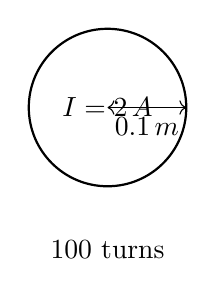
\begin{tikzpicture}[x=1cm,y=1cm]

% Circular coil (scaled correctly: radius = 0.1 m)
\draw[thick] (0,0) circle (1);
\node at (0,0) {$I=2\,A$};

% Radius marking
\draw[<->] (0,0) -- (1,0);
\node[below] at (0.5,0) {$0.1\,m$};

\node at (0,-1.8) {100 turns};

\end{tikzpicture}

A) \(0\)  

B) \(+1\%\)  

C) \(+2\%\)  

D) \(-1\%\)  

\item A series RLC circuit operates slightly above resonance frequency so that \(\omega = \omega_0(1+\epsilon)\), where \(\epsilon\) is small and positive. The phase angle between current and voltage is small but nonzero, and impedance is dominated by difference of reactances. The circuit behaves predominantly:  

A) Inductive because \(X_L>X_C\)  

B) Capacitive because \(X_C>X_L\)  

C) Resistive because \(R\) dominates  

D) At maximum current condition  

\item A charged particle moves perpendicular to uniform magnetic field with constant speed. A weak electric field parallel to velocity is introduced such that electric force equals \(1\%\) of magnetic force at that instant. Over one complete cyclotron period, the fractional change in kinetic energy is approximately:  

A) \(0\)  

B) \(1\%\)  

C) \(2\pi\%\)  

D) Second-order small  

\item In a transformer under load, leakage inductance produces additional reactance proportional to frequency. If load current amplitude remains fixed while supply frequency doubles, the leakage voltage drop amplitude becomes:  

A) unchanged

B) twice  

C) four times  

D) half  

\item During total internal reflection at a glass–air interface, angle of incidence exceeds critical angle by small amount \(\delta\). Penetration depth of evanescent field varies inversely with square root of excess term. If \(\delta\) is doubled (small-angle limit), penetration depth approximately:  

A) halves  

B) doubles  

C) unchanged  

D) decreases by factor \(\sqrt{2}\)  

\item Magnetic energy stored in an inductor is \(U=\frac12 LI^2\). If current increases by \(3\%\) while inductance decreases by \(1\%\) simultaneously, and second-order terms are neglected, the fractional change in stored magnetic energy equals:  

A) \(+5\%\)  

B) \(+4\%\)  

C) \(+3\%\)  

D) \(+2\%\)  

\end{enumerate}

\end{document}